\documentclass[a4paper, 12pt, twoside]{article}
\usepackage[T2A,T1]{fontenc}
\usepackage[utf8]{inputenc}
\usepackage[english, russian]{babel}
\usepackage{graphicx}
\usepackage[hcentering, bindingoffset = 10mm, right = 15 mm, left = 15 mm, top=20mm, bottom = 20 mm]{geometry}
\usepackage{multirow}
\usepackage{ gensymb }
\usepackage{lipsum}
\usepackage{amsmath, amstext}
\usepackage{siunitx}
\usepackage{subcaption}
\usepackage{wrapfig}
\usepackage{adjustbox}
\usepackage{enumerate, indentfirst, float}
\usepackage{capt-of, svg}
\usepackage{ctable}

\newcommand*{\hm}[1]{#1\nobreak\discretionary{} 
	{\hbox{$\mathsurround=0pt #1$}}{}}
\usepackage{cmap} % Улучшенный поиск русских слов в полученном pdf-файле

\usepackage{pscyr} % Нормальные шрифты
\usepackage[normalem]{ulem} % для подчёркиваний uline
\ULdepth = 0.16em

\usepackage{fancyhdr} %Колонтикулы
\pagestyle{fancy}
\lhead{
\includegraphics[width = 10 mm]{logo.jpg} Лабораторная работа № 4.1.2}
\rhead{\textit{15 марта 2018 г.}}

\newenvironment{bottompar}{\par\vspace*{\fill}}{\clearpage}

\begin{document}
	\begin{titlepage}
		
		\newcommand{\HRule}{\rule{\linewidth}{0.7mm}} % Defines a new command for the horizontal lines, change thickness here
		
		\center % Center everything on the page
		
		%----------------------------------------------------------------------------------------
		%	HEADING SECTIONS
		%----------------------------------------------------------------------------------------
		
		\textsc{\LARGE Московский Физико-Технический Институт}\\[1,5cm] % Name of your university/college
		\textsc{\Large Кафедра общей физики}\\[0.5cm] % Major heading such as course name
		\textsc{\large Лабораторная работа \textnumero  4.1.2}\\[0.5cm] % Minor heading such as course title
		
		%----------------------------------------------------------------------------------------
		%	TITLE SECTION
		%----------------------------------------------------------------------------------------
		
		\HRule
		\\[0.4cm]
		{ \huge \bfseries Моделирование оптических приборов и определение их увеличения}
		\\[0.2cm] % Title of your document
		\HRule
		\\[1.5cm]
		
		
		
		%----------------------------------------------------------------------------------------
		%	AUTHOR SECTION
		%----------------------------------------------------------------------------------------
		
		\begin{minipage}{0.4\textwidth}
			\begin{flushleft} \large
				\textbf{Автор:}\\
				Глеб Уваркин \\
				615 группа
			\end{flushleft}
		\end{minipage}
		~
		\begin{minipage}{0.4\textwidth}
			\begin{flushright} \large
				\textbf {Преподаватель:} \\
				Клёнов Сергей Львович % Supervisor's Name
			\end{flushright}
		\end{minipage}
		
		\begin{bottompar}
			\begin{center}
				
\includegraphics[width = 80 mm]{logo.jpg}
			\end{center}
			{\large 15 марта 2018 г.}
			
		\end{bottompar}
		\vfill % Fill the rest of the page with whitespace
		
	\end{titlepage}
	
	{\Large \uline { \textbf  {Цель работы:}}}
	
	\vspace{2mm}
	Изучение модели зрительных труб (астрономической трубы Кеплера и земной трубы Галилея) и микроскопа, определение их увеличения.
	\vspace{\baselineskip}
	
	{\Large \uline { \textbf  {В работе используются:}}}
	
	\vspace{2mm}
	
	Оптическая скамья, набор линз, экран, осветитель со шкалой, зрительная труба, диафрагма, линейка.
	
	\section{Теоретическая справка.}
	
	
	\subsection{Определение фокусных расстояний тонких линз с помощью зрительной трубы.}
	\begin{minipage}{0.49\linewidth}
		\begin{figure}[H]
			\centering
			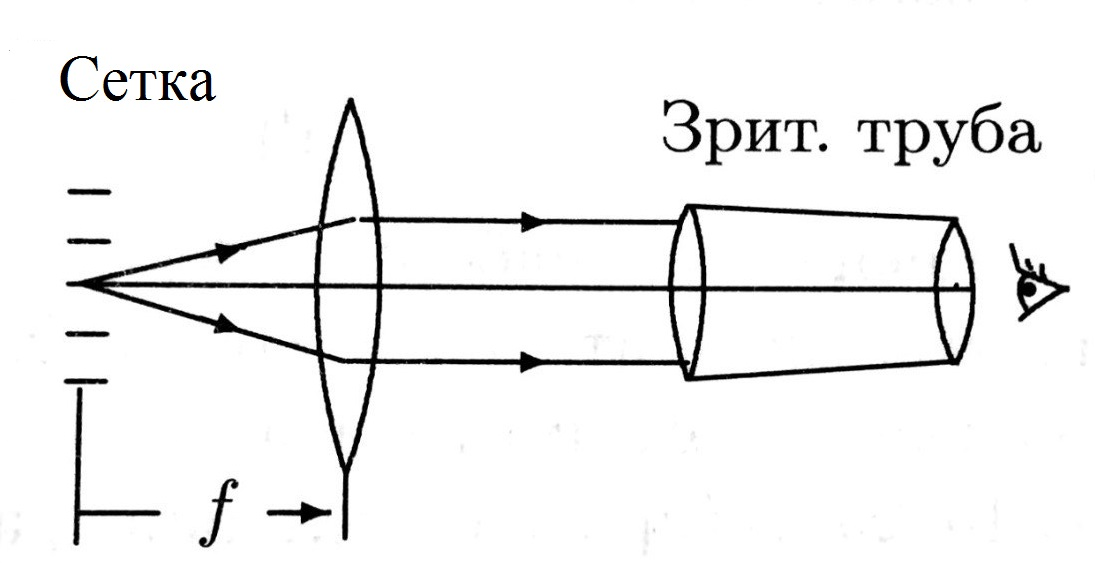
\includegraphics[width =  \textwidth]{img1}
			\caption{Определение фокусного расстояния линзы.}
			\label{img1}
		\end{figure}
	\end{minipage}
	~
	\begin{minipage}{0.49\linewidth}
		Для определения фокусных расстояний линз с помощью зрительной трубы (рис. \ref{img1}) необходимо настроить трубу на бесконечность. Передвигая линзу вдоль скамьи, получим в окуляре изображение предмета. При этом расстояние между предметом и серединой тонкой линзы равно её фокусному расстоянию.
	\end{minipage}

	\begin{minipage}{0.49\linewidth}
		\begin{figure}[H]
			\centering
			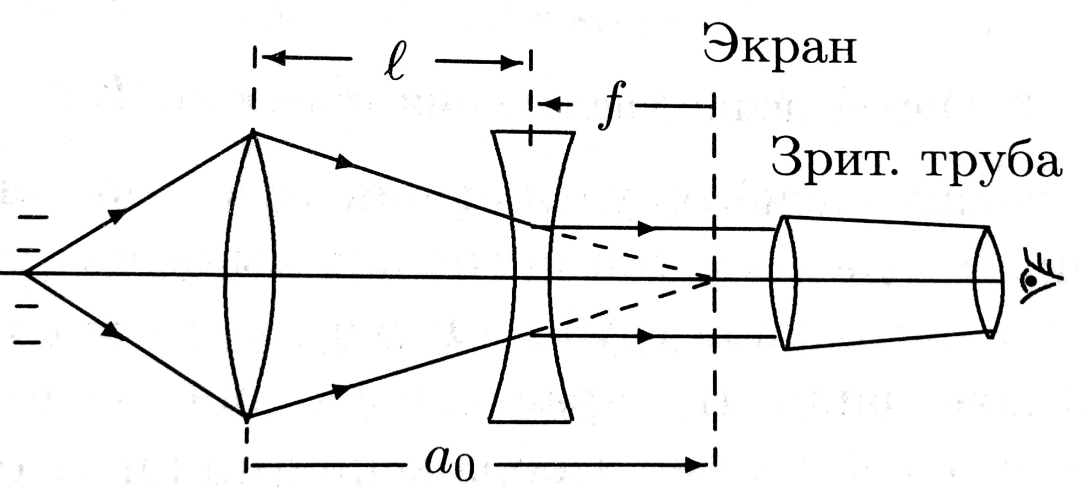
\includegraphics[width =  \textwidth]{img2}
			\caption{Определение фокусного расстояния рассеивающей линзы.}
			\label{img2}
		\end{figure}
	\end{minipage}
	~
	\begin{minipage}{0.49\linewidth}
	Для определения фокусного расстояния тонкой рассеивающей линзы получим на экране увеличенное изображение сетки при помощи одной короткофокусной собирающей линзы. Измерим расстояние $a_0$ между линзой и экраном. Измерив расстояние между линзами $l$, рассчитаем фокусное расстояние рассеивающей линзы $f = l - a_0$.
	\end{minipage}

	\subsection{Телескоп Кеплера.}
	\label{theor}
	\begin{figure}[H]
		\centering
		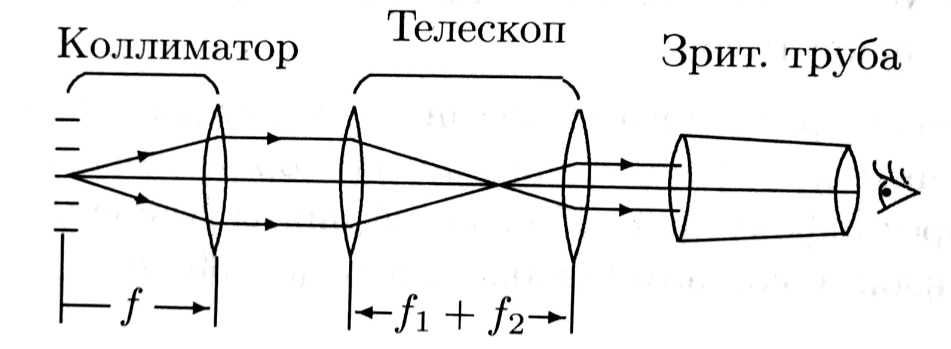
\includegraphics[width =  0.6\textwidth]{img3}
		\caption{Определение увеличения телескопа Кеплера.}
		\label{img3}
	\end{figure}
	
	Схема изучения зрительной трубы Кеплера представлена на рис. \ref{img3}. Определим размер изображения $h_1$ одного миллиметра шкалы осветителя в делениях окулярной шкалы зрительной трубы. Очевидно, что $h_1 = k ~ \mathrm{tg} \alpha_1 \approx k\alpha_1$, где $k$ -- некоторый коэффициент, характеризующий увеличение зрительной трубы, $\alpha_1$ -- угловой размер изображения миллиметрового деления шкалы осветителя, наблюдаемого через коллиматор.
	
	Соберём модель телескопа, рассчитаем увеличение исследуемой модели телескопа через отношение передних фокусных расстояний линз $f_1, f_2$ :
	
	\begin{equation}
		N_T = -\dfrac{f_1}{f_2}
	\end{equation}
	
	Определим увеличение телескопа через отношение углов, под которыми объект виден через телескоп и без него:
	
	\begin{equation}
	N_T = \dfrac{\alpha_2}{\alpha_1} = - \dfrac{h_2}{h_1},
	\end{equation}
	
	где $\alpha_2$ -- угловой размер изображения миллиметрового деления шкалы при наблюдении через телескоп, $h_2$ -- размер изображения миллиметрового деления шкалы осветителя в делениях окулярной шкалы.
	
	
	Определим увеличение телескопа, сравнив диаметр оправы его объектива и диаметр изображения этой оправы в окуляре:
	
	\begin{equation}
	N_T = \mp \dfrac{D_1}{D_2},
	\end{equation}
	
	где $D_1$ -- диаметр объектива, а $D_2$ -- диаметр его изображения.
	
	\subsection{Модель микроскопа.}
	
\begin{minipage}{0.25\linewidth}
	\begin{figure}[H]
		\centering
		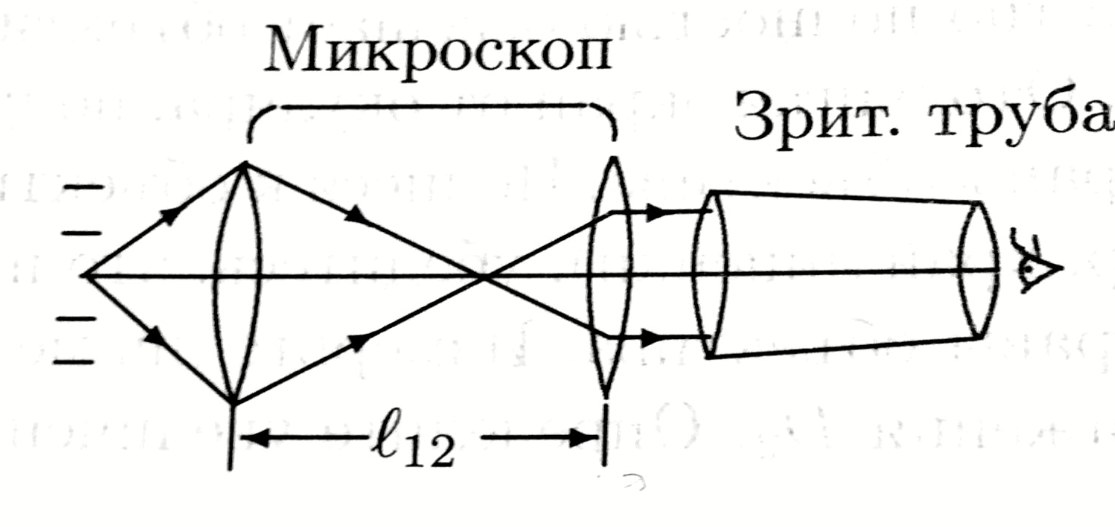
\includegraphics[width =  \textwidth]{img4}
		\caption{Модель микроскопа.}
		\label{img4}
	\end{figure}
\end{minipage}
~
\begin{minipage}{0.74\linewidth}
	Для создания модели микроскопа с увеличением $N_M = 5$ отберём самые короткофокусные собирающие линзы из набора. Рассчитаем необходимые оптический интервал $\Delta$ и длину тубуса $l_{12}$ по формулам:
	
	\begin{equation}
	\label{mictheor}
	N_M = N_1 N_2, ~~~ N_1 = -\dfrac{\Delta}{f_1}, ~~~ N_2 = \dfrac{L}{f_2}, ~~~ \Delta = l_{12} - f_1 - f_2,
	\end{equation}
	где $N_1, N_2$ -- увеличения объектива и окуляра, $f_1, f_2$ -- положительные передние фокусные расстояния линз, $L = 25~\text{см}$ -- расстояние наилучшего зрения.
\end{minipage}

~

Для экспериментального определения увеличения микроскопа измерим величину изображения $h_2$ миллиметрового деления предметной шкалы в делениях окулярной шкалы:

\begin{equation}
\label{mic}
N_M = -\dfrac{h_2}{h_1}\dfrac{L}{f}
\end{equation} 

\newpage

\section{Проведение и обработка измерений.} 

\subsection{Определение фокусных расстояний тонких линз с помощью зрительной трубы.}

Для начала отберём из набора собирающие линзы и определим "на глаз" их фокусные расстояния. Занесём результаты в таблицу \ref{t1}.

\begin{table}[H]
	\centering
	\caption{Определение фокусных расстояний собирающих линз "на глаз".}
	\label{t1}
	\begin{tabular}{c|c|c|c|c} \toprule
		№ линзы                 & 1  & 2  & 3  & 4  \\ \midrule
		Фокусное расстояние, см & 10 & 10 & 22 & 30 \\ \bottomrule
	\end{tabular}
\end{table}


Теперь определим их более точным способом, а именно с помощью зрительной трубы (рис. \ref{img1}). Результаты занесём в таблицу \ref{t2}.

\begin{table}[H]
	\centering
	\caption{Определение фокусных расстояний собирающих линз с помощью зрительной трубы.}
	\label{t2}
	\begin{tabular}{c|c|c|c|c} \toprule
		№ линзы                 & 1   & 2    & 3    & 4    \\ \midrule
		Фокусное расстояние, см & 8.0 & 10.7 & 19.0 & 27.4 \\ \bottomrule
	\end{tabular}
\end{table}

Погрешности измерений возьмём равными $0.5~\text{см}$. Она обусловлена конечной толщиной линз и случайной неточностью измерения.\\

Для 4 линзы проведём измерения, повернув её другой стороной к источнику. Получаем, что $f = 28~\text{см}$, что приблизительно совпадает с уже имеющимся значением. Отсюда делаем вывод, что линзу можно считать тонкой.\\ 


Определим фокусное расстояние рассеивающей линзы с помощью установки, показанной на рис. \ref{img2}. 

\begin{table}[H]
	\centering
	\caption{Определение фокусного расстояния рассеивающей линзы.}
	\label{t3}
	\begin{tabular}{c|c|c}\toprule
		$a_0,~\text{см}$ & $l,~\text{см}$ & $f,~\text{см}$ \\ \midrule
		23.5             & 14.0           & 9.5        \\ \bottomrule   
	\end{tabular}
\end{table}
	
\subsection{Телескоп Кеплера.}

Соберём установка, показанную на рис. \ref{img3}. Измерим расстояние между объективом и окуляром телескопа и сравним его с суммой фокусных расстояний (табл. \ref{t4}).

\begin{table}[H]
	\centering
	\caption{Расстояние между объективом и окуляром.}
	\label{t4}
	\begin{tabular}{c|c} \toprule
		$f_1+f_2,~\text{см}$ & Факт., см \\ \midrule
		38.1      & 39.5  \\ \bottomrule
	\end{tabular}
\end{table}

 Измерим увеличение телескопа различными способами, описанными в разделе \ref{theor}. Значения занесём в таблицу \ref{t6}
 
 \begin{table}[H]
 	\centering
 	\caption{Необходимые данные для определения увеличения телескопа.}
 	\label{t5}
 	\begin{tabular}{c|c|c|c|c|c} \toprule
 		$f_1,~\text{см}$ & $f_2,~\text{см}$ & $h_1,~\text{дел}$ & $h_2,~\text{дел}$ & $D_1,~\text{см}$ & $D_2,~\text{см}$ \\ \midrule
 		10.7             & 27.4             & 9                 & 24                & 3.6              & 1.4    \\ \bottomrule         
 	\end{tabular}
 \end{table}

\begin{table}[H]
	\centering
	\caption{Увеличение телескопа.}
	\label{t6}
	\begin{tabular}{c|c|c} \toprule
		$\mathbf{N_T}$ (отношение $f_1$ и $f_2$) & $\mathbf{N_T}$ (отношение углов) & $\mathbf{N_T}$ (отношение диаметров) \\ \midrule
		\textbf{2.56} $\pm ~0.13$                          & \textbf{2.67} $\pm~0.16$                  & \textbf{2.57} $\pm~0.18$     \\ \bottomrule                 
	\end{tabular}
\end{table}

\subsection{Труба Галилея.}

Соберём модель трубы Галилея, поставив в модели трубы Кеплера вместо собирающей окулярной линзы рассеивающую линзу. Измерим увеличение трубы двумя способами: через отношение передних фокусных расстояний линз $f_1$, $f_2$ и через отношение углов, под которыми объект виден через телескоп и без него. Данные занесём в таблицу \ref{t8}.

\begin{table}[H]
	\centering
	\caption{Необходимые данные для определения увеличения телескопа.}
	\label{t7}
	\begin{tabular}{c|c|c|c} \toprule
		$f_1,~\text{см}$ & $f_2,~\text{см}$ & $h_1,~\text{дел}$ & $h_2,~\text{дел}$ \\ \midrule
		27.4             & 9.5              & 9                 & 26        \\ \bottomrule       
	\end{tabular}
\end{table}

\begin{table}[H]
	\centering
	\caption{Увеличение трубы Галилея.}
	\label{t8}
	\begin{tabular}{c|c} \toprule
		$\mathbf{N_T}$ (отношение $f_1$ и $f_2$) & $\mathbf{N_T}$ (отношение углов) \\ \midrule
		\textbf{2.88} $\pm~0.16$                           & \textbf{2.88} $\pm~0.17$ \\ \bottomrule                 
	\end{tabular}
\end{table}


\subsection{Модель микроскопа.}

Соберём модель микроскопа, как показано на рис. \ref{img4}. Получим в поле зрения трубы изображение миллиметровой шкалы осветителя. С помощью формулы \eqref{mic} рассчитаем увеличения микроскопа. Данные занесём в таблицу \ref{t9}.

\begin{table}[H]
	\centering
	\caption{Увеличение микроскопа.}
	\label{t9}
	\begin{tabular}{c|c|c|c|c}\toprule
		$h_1,~\text{дел}$ & $h_2,~\text{дел}$ & $L,~\text{см}$ & $f,~\text{см}$ & $\mathbf{N_M}$ \\ \midrule
		9                 & 34                & 25.0           & 19.0           & \textbf{4.97} $\pm~0.31$ \\ \bottomrule
	\end{tabular}
\end{table}

Теперь рассчитаем увеличение микроскопа по формуле \eqref{mictheor}. Данные занесём в таблицу \ref{t10}.

\begin{table}[H]
	\centering
	\caption{Увеличение микроскопа (теория).}
	\label{t10}
	\begin{tabular}{c|c|c|c|c} \toprule
		$l_{12},~\text{см}$ & $f_1,~\text{см}$ & $f_2,~\text{см}$ & $\Delta,~\text{см}$ &$\mathbf{N_M}$ \\ \midrule
		34.0                & 8.0              & 10.7             & 15.3                & \textbf{4.47} $\pm~0.42$ \\ \bottomrule
	\end{tabular}
\end{table}

\section{Вывод.}
\begin{itemize}
	\item В результате проведения данной лабораторной работы была изучена модель зрительных труб (астрономической трубы Кеплера и земной трубы Галилея) и микроскопа, а также определено их увеличение.
	
	\item Значения увеличения, полученные разными способами, с учётом погрешности совпадают.
	
	\item Наибольшую погрешность в результат вносит неточность метода измерения расстояний между элементами приборов.
\end{itemize}
\end{document}
